% !TEX root = ../main.tex
%
\chapter{Verwandte Arbeiten}
\label{sec:related}

Die in~\ref{sec:intro:goals} beschriebenen Ziele werden bereits seit langem erforscht.
Der Begriff \textit{Wissensgraph} wurde 2012 durch Google popularisiert, die Ideen dahinter lassen sich allerdings bis ins Ende des 19. Jahrhunderts zurückverfolgen.
Dieses Kapitel zeigt auf, wie sich die Themen dieser Arbeit in die bisherige Forschung einfügen.
\ref{sec:related:kr} ordnet das Konzept des Wissensgraphen in die Entwicklungsgeschichte der Wissensrepräsentation ein.
\ref{sec:related:kbc} beschreibt die aktuell verwendeten Verfahren zur Konstruktion von Wissensgraphen.
In~\ref{sec:related:nlp} wird schließlich ein Überblick über die momentan verbreiteten NLP (\textit{natural language processing}) Werkzeuge gegeben.

\section{Ansätze zur Wissensrepräsentation}
\label{sec:related:kr}

\subsection{Logische Grundlagen}
\label{sec:related:kr:logic}

Die Entwicklung der Wissensrepräsentation hängt eng mit der Entwicklung der Logik zusammen.
Während in der formalen Logik und Mathematik die Prädikatenlogik das allgemein verwendete Kalkül ist und alternative Formalismen kaum verbreitet sind, finden im Bereich der Wissensrepräsentation bis heute diverse andere Kalküle Verwendung.
Diese werden im Folgenden kurz vorgestellt.

\paragraph{Begriffsschrift (1879)}
Gottlob Freges Buch über die \textit{Begriffsschrift} gilt als eines der bedeutsamsten Werke der Logik.
Sie ist der erste Formalismus mit der Mächtigkeit der modernen Prädikatenlogik zweiter Ordnung mit Identität.
Frege benutzt hierfür eine zweidimensionale Notation, die sich stark von der heute gebräuchlichen, linearen, an die Algebra angelehnte Notation unterscheidet.
\begin{equation*}
	\vcenter{\hbox{\Fconditional[\Fanqn{a}]{\Fcontent \mathfrak{R(a)}}{\Fncontent \mathfrak{P(a)}}}}
	\quad\Leftrightarrow\quad
	\exists\ a: P(a) \lor R(a)
\end{equation*}
Im Gegensatz zur Prädikatenlogik gibt es keine eigene Syntax für \textit{UND} und \textit{ODER};
diese Operatoren müssen durch die Kombination von Negation und Implikation abgebildet werden.
Zudem gibt es ausschließlich den Allquantor;
eine existenzquantisierte Aussage muss durch Negation der negierten allquantisierten Aussage ausgedrückt werden.

\paragraph{Prädikatenlogik: Peirce Notation (1885)}
Unabhängig von Frege entwickelte der amerikanische Mathematiker Charles Sanders Peirce ebenfalls ein prädikatenlogisches Kalkül.
Peirces Notation hatte starke Ähnlichkeiten mit der heute benutzten linearen Schreibweise.
Statt den modernen Symbolen hat Peirce allerdings die algebraischen Operatoren benutzt, um die Analogien zwischen Logik und Algebra auszudrücken.
\begin{equation*}
	\Sigma_a\ P_a + R_a
	\quad\Leftrightarrow\quad
	\exists\ a: P(a) \lor R(a)
\end{equation*}

\paragraph{Existential Graphs (1897)}
Neben seiner zuvor entwickelten linearen prädikatenlogischen Notation, hat Peirce zudem viele Jahre an einem alternativen graphischen Kalkül gearbeitet, welches er \textit{Existential Graphs} (zu dt.~Existenzgraphen) nannte.
Ähnlich wie die Begriffsschrift werden Existenzgraphen zweidimensional dargestellt.
Von dieser Gemeinsamkeit abgesehen, funktionieren sie allerdings fundamental verschieden.
Ein logischer Ausdruck wird hier durch einen ungerichteten Graphen beschrieben.
Die konkrete räumliche Anordnung der Knoten und Kanten hat dabei keine semantische Relevanz.

Peirce hat Existenzgraphen als ein dreistufiges aufeinander aufbauendes System konzipiert.
Die erste Stufe, die sog.\ $\alpha$-Graphen, umfasst alle notwendigen syntaktischen Elemente, um ein Kalkül mit der Mächtigkeit der Aussagenlogik zu erhalten.
Die $\beta$-Graphen bilden die zweite Stufe und erweitern die Syntax der $\alpha$-Graphen, sodass die Mächtigkeit der Prädikatenlogik erster Ordnung erreicht wird.
Sowohl für $\alpha$-, als auch für $\beta$-Graphen, ist die Vollständigkeit und Korrektheit bewiesen.
Die dritte Stufe ($\gamma$-Graphen) wurde von Pierce nie vollendet;
sie deckt in etwa die Mächtigkeit der heutigen Prädikatenlogik höherer Ordnung sowie der Modallogik ab.
\begin{align*}
	\vcenter{\hbox{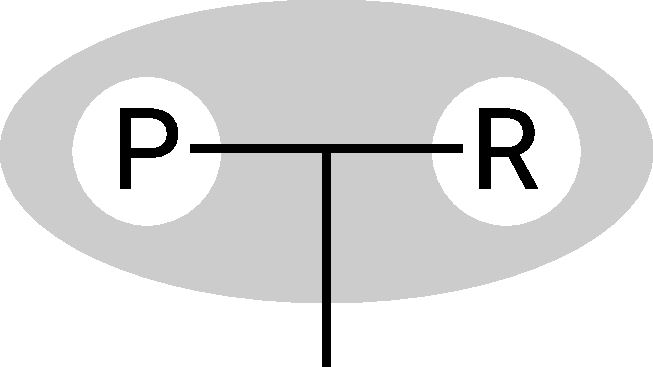
\includegraphics[height=3em]{gfx/related-work/existentialGraphExample1.pdf}}}
	\quad\Leftrightarrow\quad
	\exists\ a: P(a) \lor R(a)
\end{align*}
Wie schon die Begriffsschrift, sind Existenzgraphen syntaktisch minimal.
Direkt ausdrücken lässt sich lediglich \textit{UND}, der Existenzquantor und die Negation.
Ein weiterer Unterschied zur heutigen Prädikatenlogik ist die Beschreibung logischer Inferenzen.
Im Gegensatz zu den prädikatenlogischen Ersetzungsaxiomen, die auf der syntaktischen Struktur von logischen Ausdrücken operieren (z.~B. für Kommutativität), lassen sich die Ersetzungsaxiome für Existenzgraphen als Graphtransformationsregeln verstehen, die bestimmte Teilmengen der Knoten und Kanten eines Ausdrucks durch andere äquivalente Knoten- und Kantenmengen ersetzen.

\paragraph{Prädikatenlogik: Peano-Russell Notation (1910)}
Die zweidimensionalen Notationen wurde häufig kritisiert, da sie die lineare, algebraische Notation der symbolischen Logik von Boole und De Morgan verwarf.
Freges Begriffsschrft und Peirces Existenzgraphen konnten daher nicht durchsetzen.
Peirces algebraische prädikatenlogische Notation hingegen, stieß auf größere Akzeptanz.
Giuseppe Peano hat auf deren Basis eine ähnliche Notation entwickelt, welche allerdings nicht die algebraischen Operatoren benutzt, so dass sich logische Ausdrücke besser mit mathematischen Ausdrücken mischen lassen.
Bertrand Russell hat Peanos Notation anschließend in leicht abgewandelter Form in den \textit{Principia Mathematica} (1910) benutzt.
Diese sog.~Peano-Russell-Notation ist im Wesentlichen identisch mit der modernen Schreibweise.

Trotz des Verschwindens der zweidimensionalen Notationen, finden sich noch heute Anlehnungen daran.
So ist z.~B. die Negation $\lnot A$ auf Freges negierten Inhaltsstrich $\Fncontent A$ und der Ableitungsoperator $\vdash$ auf Freges Urteilsstrich mit angefügtem Inhaltsstrich $\Facontent$ zurückzuführen.

\subsection{Entwicklung maschineller Wissensrepräsentation}
\label{sec:related:kr:history}

Die Idee Computer zur Lösung beliebiger Probleme zu benutzen ist nicht neu.
Da ein solches maschinelles Problemlösen immer die Verfügbarkeit von Hintergrundwissen über die Problemdomäne erfordert,
wurden Methoden zur Wissensrepräsentation immer im Zusammenhang mit Problemlösern erforscht.
So wie effiziente Datenstrukturen die Implementation effizienter Algorithmen ermöglichen, ermöglichen gute Wissensrepräsentationen die Implementation guter Problemlöser.
Was genau nun als ein guter Problemlöser verstanden wird, hat sich im Laufe der Jahre allerdings immer wieder verändert.

\paragraph{Logic Theorist (1955)}
Einer der ersten maschinellen Problemlöser war der von Simon, Shaw und Newell entwickelte \textit{Logic Theorist} (LT).
LT war in der Lage logische Aussagen zu beweisen, indem er systematisch Ersetzungsaxiome auf eine gegebene Aussage angewandt hat, bis die gesuchte Lösung abgeleitet wurde.

\paragraph{General Problem Solver (1959)}
Die Grundidee des LT haben Simon, Shaw und Newell wenige Jahre später im \textit{General Problem Solver} (GPS) erweitert.
Es wurden Heuristiken hinzugefügt, um den Suchraum geschickter zu durchlaufen.
GPS war ein universeller Problemlöser, konnte also jedes Problem lösen, das sich durch eine Menge von Horn-Klauseln ausdrücken lässt.
Zwar war es so prinzipiell möglich Probleme aus diversen Domänen zu lösen, aufgrund der kombinatorischen Explosion war GPS alledings nicht zur Lösung praktischer Probleme geeignet.

\paragraph{Expertensysteme (1970)}
Aufgrund der Misserfolge universeller Problemlöser für praktische Probleme, hat die Forschung begonnen sich mehr auf die Entwicklung von Expertensystemen zu fokussieren.

\paragraph{Conceptual Graphs (1976)}

\subsection{Aktuelle Wissensrepräsentationsansätze}
\label{sec:related:kr:today}

\subsubsection{Semantic Web}
\label{sec:related:kr:today:sw}

\subsubsection{NELL}
\label{sec:related:kr:today:nell}

\subsubsection{Google Knowledge Graph}
\label{sec:related:kr:today:google-kg}

\section{Konstruktionsansätze für Wissensgraphen}
\label{sec:related:kbc}

\section{NLP Werkzeuge}
\label{sec:related:nlp}
